\begin{frame}{}
    \begin{center}
        \large \textbf{BERT (Bidirectional Encoder Representations from Transformers)}
    \end{center}
    \vspace{20pt}
    
    \textbf{Author(s):}
    \begin{itemizeSpaced}{5pt}
    {\color{DimGrey} 
    
        \item Devlin et al. (2019) in \emph{BERT: Pre-training of Deep Bidirectional Transformers for Language Understanding}
        
        \item Clark et al. (2019) in \emph{What Does BERT Look At? An Analysis of BERT's Attention}
        
        \item Wiedemann et al. (2019) in \emph{Does BERT Make Any Sense? Interpretable Word Sense Disambiguation with Contextualized Embeddings}
        
        \item Munikar et al. (2019) in \emph{Fine-Grained Sentiment Classification Using BERT}
        
    }
    \end{itemizeSpaced}
\end{frame}

% -------------------------------------------------




\begin{frame}{BERT: Motivation} 
    
    \begin{itemizeSpaced}{7pt}
        \footnotesize 
        
        \pinkbox \textbf{Problem with ELMo: } shallowly combines ``independently-trained" biLMs
        
        \item \textbf{Problem with OpenAI GPT: }unidirectional model $\Rightarrow$ gets no bidirectional context $\Rightarrow$ does poorly on \emph{sentence-level} and \emph{token-level} tasks (question answering (QA))

        
        \pinkbox \textbf{BERT's Solution: } train ``deep bidirectional representations from unlabeled text by jointly conditioning on both left and right context in all layers” (Devlin et al., 2019).
    \end{itemizeSpaced}
    
\end{frame}


\begin{frame}{BERT: Input Embeddings}
    
    \begin{itemizeSpaced}{10pt}
        \footnotesize 
        
        \pinkbox  \textbf{\textit{WordPiece} token embeddings: } \emph{WordPiece} tokenization subdivides words to smaller units 
        
        \vspace{7pt}
        \begin{itemizeSpaced}{7pt}
        
            \footnotesize
            \item to handle rare, unknown words (Weng, 2019) and reduce vocabulary size while increasing amount of data available per word.
            
            \pinkbox \textbf{Example: }if \texttt{"play"} and \texttt{"**ing"} and \texttt{"**ed"} are present in the vocabulary but \texttt{"playing"} and \texttt{"played"} are not, then these can be recognized by their sub-units. 
        \end{itemizeSpaced}
        
        
        \item \textbf{Segment embeddings: } are arbitrary spans of text (packing sentence parts). 
        NOTE: Transformer-XL respects sentence boundaries. 
        
        \item \textbf{Positional embeddings: } as in ordinary Transformer (to inject word order information). 
    
    \end{itemizeSpaced}
    
\end{frame}




\begin{frame}{BERT Framework: MLM and NSP}

\linespread{0.3} 

BERT does \textbf{pre-training} (trains on \emph{unlabeled data} using MLM and NSP), and \textbf{fine-tuning} (to use pre-training parameters to train over \emph{labeled data} for nlp tasks)


{\small \textbf{Masked language model (MLM): }}
    \begin{itemizeSpaced}{5pt}
        \pinkbox \textbf{Motivation: } bidirectional conditioning causes information leakage (a word can implicitly ``see itself" letting the model trivially guess the target word in a multi-layered context (Devlin et al., 2019)). 
        
        \item \textbf{Goal: }randomly masks some input tokens to predict original masked word using only its context. 
        
        \item \textbf{Effect of MLM: } fuses left and right context to get \emph{deep} bidirectional context (unlike ELMo's shallow left-to-right language model (Devlin et al., 2019)).  
    \end{itemizeSpaced}
    
{\small \textbf{Next Sentence Prediction (NSP):}}
    \begin{itemizeSpaced}{5pt}
        \pinkbox \textbf{Motivation: } to capture \emph{sentence-level} information $\Rightarrow$ to do well in question-answering (QA) and natural language inference (NLI) tasks
        
        
        \item \textbf{Goal: } task that finds if sentence is the next sentence of the other. 
        
    \end{itemizeSpaced}
    
\end{frame}


% \begin{frame}{BERT: General Experimental Results}
% 
%     \begin{itemizeSpaced}{2pt}
%         \item Using a simple accuracy measure, Munikar et al. (2019) found that a pre-trained BERT model fine-tuned for \textbf{sentiment analysis (SA)} task outperformed complex models (RNN, CNNs).
%         
%         \pinkbox This proves \textbf{transfer learning} is possible with BERT's deep contextual bidirectional language model. 
%     \end{itemizeSpaced}
% 
% 
% 
%     \begin{table}[ht!]
%       \centering
%       \vspace{-7pt}
%       
%       \begin{tabular}{ c }
%       
%         \begin{minipage}{.7\textwidth}
%           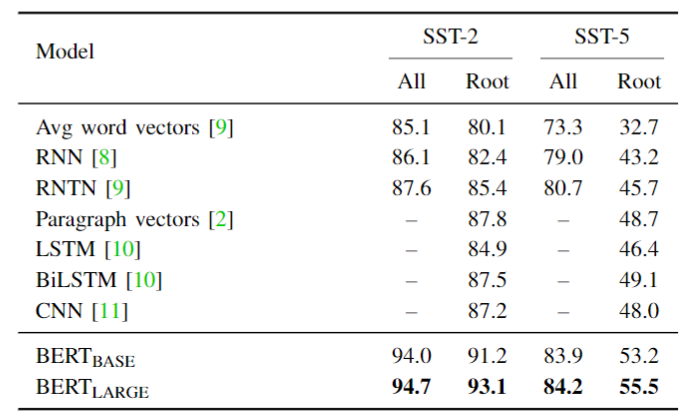
\includegraphics[width=\linewidth]{imgs/table_bert_vsOtherModels.png}
%         \end{minipage}
%         \vspace{-7pt}
%       
%       \end{tabular}
%       
%       \caption{\linespread{0.3} \footnotesize Accuracy (\%) of several models on \textbf{sentiment classification (SC)} SST dataset. BERT has highest accuracy scores. From \emph{Table B.II in Fine-Grained Sentiment Classification Using BERT}, by Munikar et al., 2019. \url{https://arxiv.org/pdf/1910.03474.pdf}. Copyright 2019 by Munikar et al.}
%       \label{tbl:bertExperimentResults}
%       \vspace{-10pt}
%     \end{table}
%     
% \end{frame}



\begin{frame}{Probing BERT: BERT Learns Dependency Syntax}


    \begin{columns}
        
        \begin{column}{0.6\textwidth}
            %\vspace{\topsep}
            \vspace{5pt}
            \begin{center}
            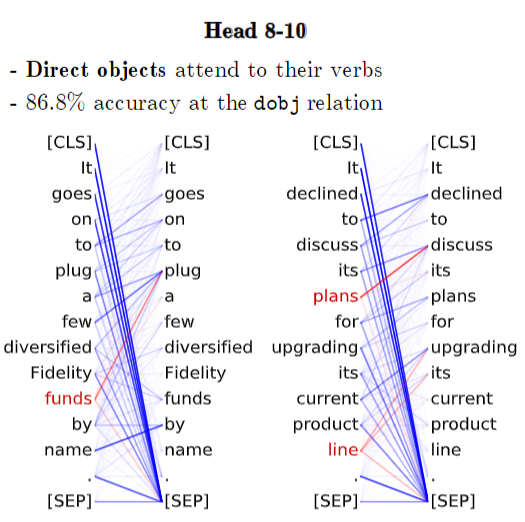
\includegraphics[width=0.8\columnwidth]{imgs/bert_headsDirectObject.png}
            \end{center}
            \vspace{-10pt}
            
            \captionof{figure}{\tiny \linespread{0.2} BERT attention heads capture syntax. In heads 8-10, direct objects are found to attend to their verbs. Line darkness indicates attention strength. Red indicates attention to/from red words, to highlight certain attentional behaviors. From \emph{What Does BERT Look At? An Analysis of BERT's Attention}, by Clark et al., 2019. \url{https://arxiv.org/abs/1906.04341}. } 
            \label{fig:bertHeadDirectObject}
        \end{column}
        
        \begin{column}{0.4\textwidth}
        
            Clark et al. (2019) found ...\newline
            
            \begin{itemizeSpaced}{10pt}
            
                %\scriptsize
                %\item  While BERT's attention heads do not capture syntax dependency structure as a whole....
            
                %\item ... different heads are better at detecting different syntax dependency relationships.
                
                \pinkbox BERT's attention heads detect ``direct objects of verbs, determiners of nouns, objects of prepositions, and objects of possessive pronouns with > $75 \%$ accuracy."
                
                \item Attention heads 8-10 in \cref{fig:bertHeadDirectObject} learn how direct objects attend to their verbs. 
                
                \item BERT learns this using only \textit{self-supervision}. 
            \end{itemizeSpaced}
        \end{column}
    
    \end{columns}


\end{frame}





\begin{frame}{Probing BERT: BERT's Limitation in Segment Representation}
    
    \begin{itemizeSpaced}{10pt}
        \item BERT does not use separator tokens (\texttt{[SEP]}) to gather segment-level information. 
        
        \pinkbox BERT uses \texttt{[SEP]} as ``no-op" or stub operations for attention heads when the head is not needed for a current task. 
        
        \item How? Why? Authors investigated in two ways ...
        
        \begin{itemizeSpaced}{10pt}
        
            \item If this were true, attention heads processing \texttt{[SEP]} should attend broadly over entire segment to make the segment vectors. But in \cref{fig:bertHeadDirectObject}, heads 8-10 show direct objects attend to their verbs, and all other words attend to the \texttt{[SEP]} token. 
            
            \item Gradient measures: show much the attention to a token would change BERT's outputs. Attention to \texttt{[SEP]} increases in layers 5-10 (\cref{fig:bertSEPAttention}), WHILE the gradients for attention to \texttt{[SEP]} decrease here (\cref{fig:bertGradient})  $\Rightarrow$ attending to \texttt{[SEP]} does not significantly change BERT's outputs. 
        \end{itemizeSpaced}
    \end{itemizeSpaced}
    


So, BERT's attention heads attend to \texttt{[SEP]} when they have no other job, not to gather segment-level information. 

\textbf{Transformer-XL} by design improves this.

\end{frame}





\begin{frame}{Probing BERT: BERT's Limitation in Segment Representation}
    
    \vspace{10pt}

    \begin{figure}
    \centering
    \begin{minipage}{.47\textwidth}
      \centering
      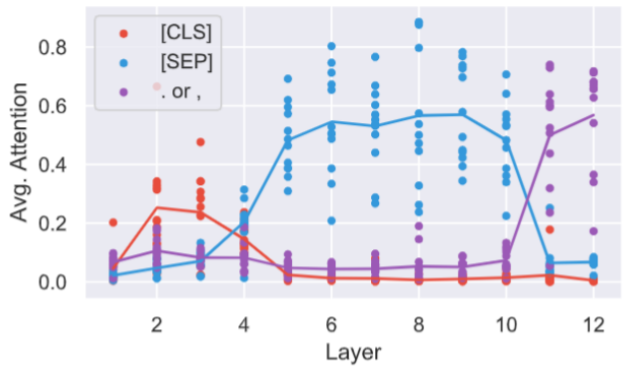
\includegraphics[width=\textwidth]{imgs/bert_attentionSEP_singleimage.png}
      \vspace{-10pt}
      \captionof{figure}{\linespread{0.1} BERT's attention heads in layers 6-10 spend more than half the average attention to separator tokens; deep heads attend to punctuation, while middle heads attend to \texttt{[SEP]}, and early heads attend to \texttt{[CLS]}. From \emph{What Does BERT Look At? An Analysis of BERT's Attention}, by Clark et al., 2019. \url{https://arxiv.org/abs/1906.04341}. Copyright 2019 by Clark et al.}
      \label{fig:bertSEPAttention}
    \end{minipage} \hspace{2em}%
    \begin{minipage}{.47\textwidth}
      \centering
      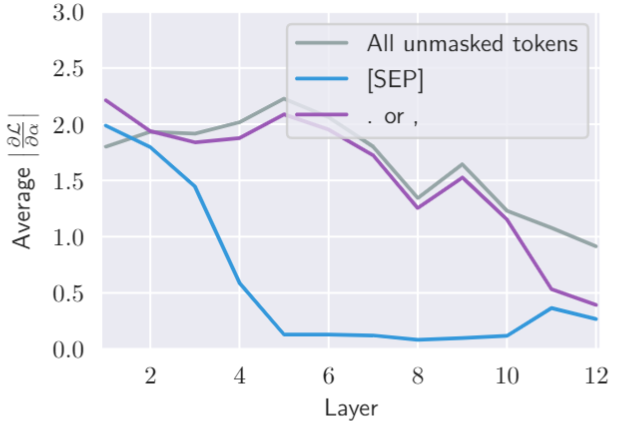
\includegraphics[width=\textwidth]{imgs/bert_attentionheads_gradient.png}
      \vspace{-15pt}
      \captionof{figure}{\linespread{0.1} Gradient-based estimates for attention to separator and punctuation tokens. Authors ``compute the magnitude of the gradient of the loss from the masked-language model (MLM) task with respect to each attention weight." From \emph{What Does BERT Look At? An Analysis of BERT's Attention}, by Clark et al., 2019. \url{https://arxiv.org/abs/1906.04341}. Copyright 2019 by Clark et al.}
      \label{fig:bertGradient}
    \end{minipage}
    \end{figure}

    
\end{frame}



\begin{frame}{BERT's Attempt at Polysemy}
    
    \vspace{15pt}
    
    \begin{itemizeSpaced}{7pt}
    
        \item ELMo and BERT were compared on \textbf{word sense disambiguation (WSD)} task $\Rightarrow$ BERT more strongly separates polysemic word senses while ELMo cannot. 
        
        \item BERT did well when the text had ...
        \vspace{5pt}
        \begin{itemizeSpaced}{7pt}
            \item \textit{vocabulary overlap}  \texttt{"along the bank of the river"} (input text) and \texttt{"along the bank of the river Greta"} (nearest neighbor found by BERT). 
            
            \item \textit{semantic overlap} \texttt{"little earthy bank”} (input) and \texttt{"huge bank [of snow]”} (nearest neighbor found by BERT)
        \end{itemizeSpaced}
        
        \item BERT struggled when text had \emph{vocabulary and semantic overlap at the same time}
        
        \begin{itemizeSpaced}{7pt}
        
            %\item \underline{False prediction 1}: BERT predicted \texttt{"land bank" as in a \emph{supply or stock} while the correct sense of \texttt{"land bank" was \emph{financial institution}
            
            \item \underline{False prediction 1}: correct word sense of \texttt{"balloon"} is a verb while BERT predicted a noun sense, so it did not even get the word class correct.
            
            \item \underline{False prediction 2}: correct sense of \texttt{"watch"} was \emph{to look attentively} while BERT predicted its sense as \emph{to follow with the eyes or the mind; observe}. 
        \end{itemizeSpaced}
        
    \end{itemizeSpaced}
    
\end{frame}